\section{Аналитический раздел}
 
\subsection{Постановка задачи}

Рассмотрим задачу рекомендательной системы новостей. На вход алгоритм получает данные о прочитанных ранее пользователям новостях. Выходом рекомендательной системы являются новости, рекомендованные к прочтению. Таким образом, задача рекомендации новостей представляет собой анализ ранее прочитанных пользователем новостей и рекомендации новостей на их основе.

Постановка задачи рекомендательной системы новостей представлена на рисунке \ref{idef0_small}. 

\begin{figure}[H]
	\centering
	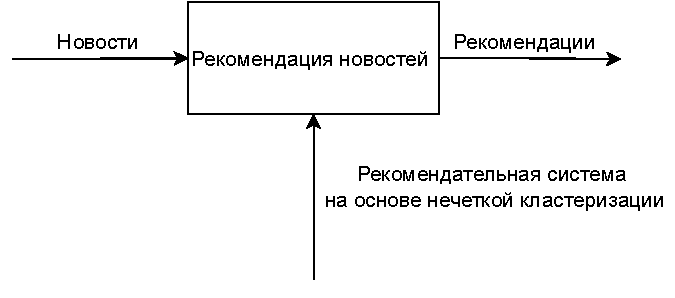
\includegraphics[width=\textwidth]{img/idef0_small.pdf}
	\caption{Постановка задачи. Диаграмма верхнего уровня}
	\label{idef0_small}
\end{figure}  

\subsection{Рекомендательная система}

Рекомендательная система — это очень большая поддоменная область интеллектуального анализа данных. Выделяются два основных вида рекомендательных систем: персонализированная и неперсонализированная. Неперсонализированная рекомендательная система — это система, делающая рекомендации на основе рейтинга элемента. Преимуществом данного вида является простота реализации. Однако, предпочтения отдельного пользователя не учитываются, следовательно, сделанная рекомендация с маленько вероятностью понравится большей части пользователей.

Другой вид — персонализированная рекомендательная система учитывает предпочтения каждого пользователя, поэтому работает эффективнее. Такие системы основаны на расчете сходства между пользователями или элементами. Для построение персонализированной рекомендательной системы существует в основном два метода: фильтрация на основе содержания (контентная фильтрация) и коллаборативная фильтрация. \cite{RecSys}

\subsection{Обучение без учителя}

Обучение без учителя использует алгоритмы машинного обучения для анализа и кластеризации немаркированных наборов данных. Эти алгоритмы обнаруживают скрытые шаблоны или группы данных без необходимости вмешательства человека. Способность алгоритмов обнаруживать сходства и различия в информации делает их идеальным решением для исследовательского анализа данных, сегментации данных и рекомендаций на их основе. 

Обучение без учителя используется в основном, для трех задач --- кластеризации, ассоциации и уменьшения размерности. Ниже будет приведено описание кластеризации и уменьшения размерности и выделены общие алгоритмы и подходы для эффективной работы с ними.

\subsubsection{Кластеризация}
Кластеризация --- это мощный инструмент машинного обучения для обнаружения структур и закономерностей в размеченных и неразмеченных наборах данных. Алгоритмы кластеризации используются для обработки необработанных, неклассифицированных объектов данных в группы, представленные структурами или шаблонами.

Цель кластерного анализа заключается в разделении объектов на группы
с учетом сходств объектов. Кластеризацию можно считать наиболее важным
методом обучения без учителя. Как и любой другой метод обучения без
учителя, кластеризация не использует идентификаторы класса для выявления
основной структуры в сборе данных. Кластер может быть определен как
совокупность объектов, которые являются подобными друг для друга и
неподобными для объектов, принадлежащих другим кластерам. Определение
кластера может быть сформулировано по-разному, в зависимости от цели
кластеризации. Можно дать общее определение кластера, согласно которому
кластер представляет собой группу объектов, которые больше подобны друг
другу, чем представителям других кластеров. Термин «подобие» может быть
истолкован как математическое подобие, измеряемое в некотором
определенном смысле. В метрических пространствах подобие часто
определяется с помощью нормы расстояния или меры расстояния. Данные
могут формировать кластеры с различными геометрическими формами,
размерами и плотностями, как показано на рис. 1.2. Кластеры могут быть
сферическими, вытянутыми и полыми.

\begin{figure}[H]
	\centering
	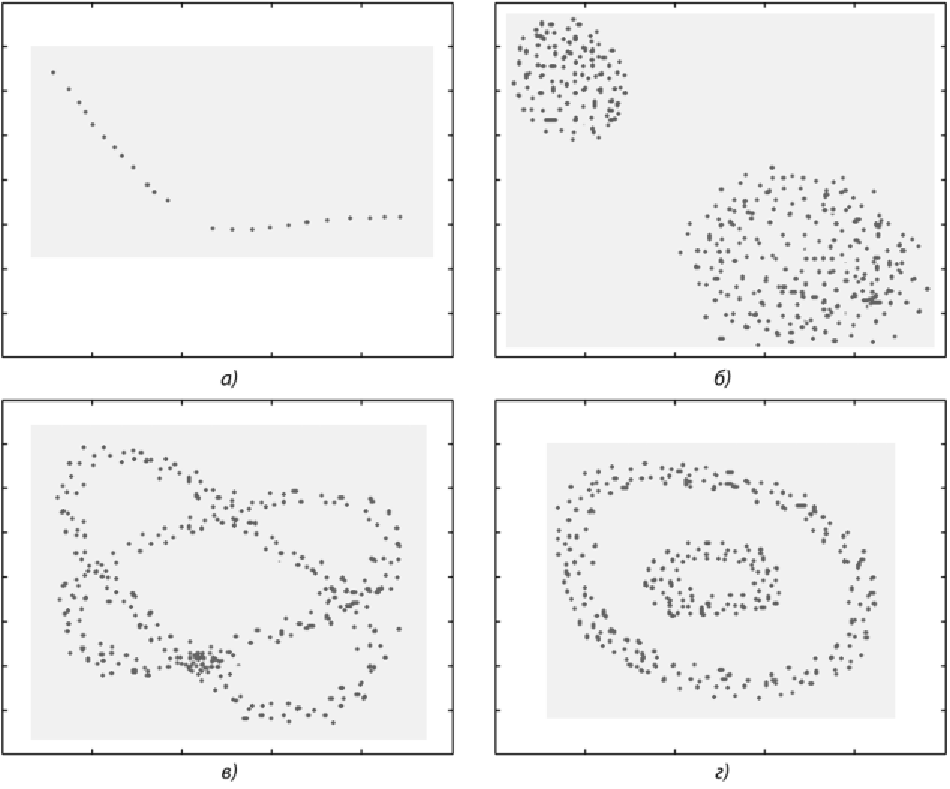
\includegraphics[width=\textwidth]{img/clusters.pdf}
	\caption{Различные формы кластеров в $R^{2}$: \textit{а} — вытянутые кластеры; \textit{б} — сферические кластеры; \textit{в}, \textit{г} — полые кластеры}
	\label{clusters}
\end{figure}  

Кластеры могут существовать в любом д-мерном пространстве.
Кластеры \textit{а}, \textit{в} и \textit{г} можно охарактеризовать как линейные и нелинейные
подпространства в пространстве данных (в данном случае $R^{2}$). Алгоритмы
кластеризации способны обнаруживать подпространства в пространствах
данных, поэтому они надежны для идентификации. \cite{ClustMethods}

Эффективность большинства алгоритмов кластеризации зависит не
только от геометрической формы и плотности отдельных кластеров, но и от
положения в пространстве и расстояния между кластерами. Кластеры могут
быть разделены, связаны друг с другом или наложены друг на друга.
Существует множество методов кластеризации, которые можно
классифицировать как четкие и нечеткие. Четкиe методы кластеризации
разбивают исходное множество объектов на несколько непересекающихся
подмножеств. При этом любой объект принадлежит только одному кластеру.
Нечеткие методы кластеризации позволяют одному и тому же объекты
принадлежать одновременно нескольким (или даже всем) кластерам, но с
различной степенью принадлежности. Нечеткая кластеризация во многих
ситуациях более “естественна”, чем четкая, например, для объектов
расположенных на границе кластеров. \cite{FuzzyClust}

\subsubsection{Нечеткая кластеризация}

Нечеткая кластеризация (вероятностная) это метод, который помогает решать задачи оценки плотности. При нечеткой кластеризации точки данных группируются на основе вероятности их принадлежности к определенному распределению. Модель Гауссовой смеси (GMM) является одним из наиболее часто используемых вероятностных методов кластеризации.

Применение нечеткой кластеризации в качестве метода для рекомендательной
системы новостей является актуальной задачей, так как каждый человек имеет
свои предпочтения в прочтении новостей, вследствие чего он хочет видеть в
рекомендациях новости, которые он хотел бы прочитать, но проблема состоит в
том, что при использовании обычной кластеризации, где отсутствует связь
кластеров, пользователю в скором времени начнут предлагаться новости одного
типа, когда как при использовании нечеткой кластеризации пользовательские
рекомендации бы обладали большей гибкостью. \cite{NewsClust}

\subsubsection{Принцип понижения размерности}

Производительность алгоритмов машинного обучения может ухудшиться при слишком большом количестве входных переменных.

Если ваши данные представлены с помощью строк и столбцов, то входные переменные — это столбцы, которые передаются в качестве входных данных модели для прогнозирования целевой переменной. Столбцы данных можно рассматривать как измерения в n-мерном пространстве признаков, а строки данных как точки в этом пространстве. В таком случае набор данных, обладает геометрической интерпретацией.

Наличие большого количества измерений в пространстве признаков может означать, что объем этого пространства очень велик, и, в свою очередь, точки, которые у нас есть в этом пространстве (строки данных), часто представляют собой небольшую и нерепрезентативную выборку. Это может существенно повлиять на производительность алгоритмов машинного обучения, подходящих для данных со многими входными характеристиками, обычно называемых «проклятием размерности». Поэтому зачастую прибегают к уменьшению количества входных признаков.

Многомерность может означать сотни, тысячи или даже миллионы входных переменных. Меньшее количество входных измерений часто означает соответственно меньшее количество параметров или более простую структуру в модели машинного обучения, называемую степенями свободы. Модель со слишком большим количеством степеней свободы, будет переобучаться на обучающем наборе данных и, следовательно, может плохо работать с новыми данными и предсказывать неправильный результат. В данном случае и прибегают к методам понижения размерности, которые, тем не менее, хорошо обобщают набор входных данных. Одними из основных методов понижения размерности являются метод главных компонент (PCA) и метод сингулярного разложения (SVD). Ниже будет приведено изложение данных методов.

\subsubsection{Метод главных компонент (PCA)}

Метод главных компонент (PCA) --- это тип алгоритма уменьшения размерности, который используется для уменьшения избыточности и сжатия наборов данных посредством извлечения признаков. Этот метод использует линейное преобразование для создания нового представления данных, что дает набор «основных компонентов». Первый главный компонент --- это направление, которое максимизирует дисперсию набора данных. Второй главный компонент также обнаруживает максимальную дисперсию данных, но совершенно не коррелирует с первым главным компонентом, что дает направление, перпендикулярное или ортогональное первому компоненту. Этот процесс повторяется в зависимости от количества измерений, где следующий главный компонент является направлением, ортогональным предыдущим компонентам с наибольшей дисперсией.

\subsubsection{Метод сингулярного разложения (SVD)}

Метод сингулярного разложения (SVD) --- это подход к уменьшению размерности, который раскладывает матрицу $A$ на три матрицы низкого ранга. SVD приведено в формуле \ref{SVD_formula}.

\begin{equation}
\label{SVD_formula}
A = USV^T,
\end{equation}

где $U$ и $V$ --- ортогональные матрицы. $S$ --- диагональная матрица, а значения $S$ считаются сингулярными значениями матрицы $A$. Подобно PCA, он обычно используется для уменьшения шума и сжатия данных.

Сингулярное разложение является удобным методом при работе с матрицами. Оно показывает геометрическую структуру матрицы и позволяет наглядно представить имеющиеся данные. Сингулярное разложение используется при решении самых разных задач --- от приближения методом наименьших квадратов и решения систем уравнений до сжатия изображений. При этом используются разные свойства сингулярного разложения, например, способность показывать ранг матрицы, приближать матрицы данного ранга. SVD позволяет вычислять обратные и псевдообратные матрицы большого размера, что делает его полезным инструментом при решении задач регрессионного анализа.

\subsection{Обработка естественных языков}

Обработка естественного языка (Нейролингвистическое программирование (NLP)) относится к области компьютерных наук, в частности к области искусственного интеллекта или ИИ. Ее цель заключается в предоставлении компьютерам возможности понимать текст и произносимые слова почти так же, как люди.

Обработка естественного языка сочетает в себе вычислительную лингвистику --- моделирование человеческого языка на основе правил --- со статистическими моделями, машинным обучением и моделями глубокого обучения. Вместе эти технологии позволяют компьютерам обрабатывать человеческий язык в виде текстовых или голосовых данных и «понимать» его полное значение, включая намерения и чувства говорящего или пишущего. Она управляет компьютерными программами, которые переводят текст с одного языка на другой, реагируют на голосовые команды и быстро резюмируют большие объемы текста --- даже в режиме реального времени.

Для использования текста в алгоритмах машинного обучения, первоначально следует обработать сам текст, а именно произвести токенизацию, после чего произвести стемминг или лемматизацию.

\subsubsection{Токенизация}

Токенизация --- это первый шаг при разработке NLP приложения. Токенизатор разбивает неструктурированные данные и текст на естественном языке на фрагменты информации, которые можно рассматривать как отдельные элементы. Вхождения токена в документе можно использовать непосредственно как вектор, представляющий этот документ. Токенизация превращает неструктурированную строку (текстовый документ) в числовую структуру данных, пригодную для машинного обучения. 

Существуют различные инструменты токенизации текста, каждый из которых подходит под определенные задачи, основными токенизаторами являются: NLTK, TextBlob, spacy, gensim и Keras.

\subsubsection{Стемминг}

Стемминг является более простым подходом, по сравнению с лемматизацией. Это способ подготовки текста для использования в модели машинного обучения, сокращение слов до своих грамматических основ (основа слова "Африки" – "Африк"). Основа слова --- стем, не обязательно совпадает с корнем, он может включать и суффиксы. Это неизменяемая при склонении часть.

Алгоритмы стемминга обычно основаны на правилах: слово проходит через ряд условных предложений, которые определяют, как его сократить. Например, существует правило суффиксов: в английском языке «-ed» и «-ing» отрезают, чтобы сопоставить "cooking" и "cooked" с одной и той же основой "cook".

Поскольку стемминг обычно основан на эвристике, он далек от совершенства. Данный подход обладает такими недостатками как перестемминг и недостемминг.

Перестемминг (англ. overstemming) происходит, когда слишком большая часть слова обрезается. Это может привести к бессмысленным стемам, где значение слова потеряно. Или же к тому, что совершенно неродственные слова будут приведены к одной и той же основе.

Недостемминг — противоположная проблема. Подобная ситуация возникает, когда у нас есть несколько слов, которые на самом деле являются формами друг друга, но их основа слова (stem), оказываются отличными.

\subsubsection{Лемматизация}

Лемматизация --- объединение слов с одним и тем же корнем или леммой, но с разными склонениями или производными значения для дальнейшего анализа как элемента. Цель состоит в том, чтобы выявить присутствие слова в любой из его форм в текстовом блоке (корпусе) и, например, определить частоту его появления.

Подобный подход является более мощным инструментом, так как учитывает морфологический анализ слов. Он возвращает лемму, которая является базовой формой всех ее флективных форм. Для создания словарей и поиска правильной формы слова необходимы глубокие лингвистические знания. Стемминг --- это общая операция, а лемматизация --- интеллектуальная операция, в которой правильная форма будет выглядеть в словаре. Следовательно, лемматизация помогает в формировании лучших возможностей машинного обучения.

\subsubsection{Векторизация текстовых данных}

Векторизация --- процесс конвертации текста в числа. После предобработки данных, следует шаг векторизации.На данном шаге требуется закодировать текстовые данные в виде чисел, которые в дальнейшем будут использованы в алгоритмах.

Наиболее часто используемыми векторизаторами являются:

\begin{itemize}
	\item векторизация методом мешка слов (Bag of words (BOW));
	\item векторизация методом TF-IDF;
	\item векторизация методом word embedding (векторное представление слов).
\end{itemize}

Описание каждого из приведенных в списке выше векторизаторов приведено ниже.

\subsubsection{Векторизация методом мешка слов (Bag of words (BOW))}

Модель мешка слов является одной из самых простых методик векторизации текста. Данный метод создает словарь уникальных слов в корпусе (собрание всех токенов в данных), после чего создается таблица в которой столбцы соответствуют входящим в корпус уникальным словам, а строки предложениями, далее происходит инициализация ячеек 0 если слова в предложении нет и 1 иначе.

\subsubsection{Векторизация методом TF-IDF}

Векторы слов с использованием данного метода высчитываются из двух коэффициентов, а именно Term Frequency (Частота слова) и Inverse Document Frequency (Обратная частота документа).

Term Frequency высчитывает вероятность встретить слово в документе, по сравнению с общим количеством слов в документе. Пример для терма $w_i$ в документе $d_j$ приведен в формуле \ref{TF_formula}.

\begin{equation}
\label{TF_formula}
\text{Term Frequency}(w_i, d_j) = \frac{\text{количество } w_i \text{ в } d_j}{\text{количество термов в } d_j}
\end{equation}

Inverse Document Frequency (обратная частота документов) отражает долю документов в корпусе, содержащих этот термин. Слова, уникальные для небольшого процента документов (например, термины технического жаргона), получают более высокие значения важности, чем слова, общие для всех документов, к примеру местоимения, если они не были удалены на предобработке. Вычисление IDF приведено в формуле \ref{IDF_formula}.

\begin{equation}
\label{IDF_formula}
\begin{matrix}
\text{Inverse Document Frequency} =\\
 =\log{(\frac{\text{количество вхождений
			 терма в документ}}{\text{количество документов, которые содержат терм в корпусе}})}
\end{matrix}
\end{equation}

Итоговая формула \ref{TF_IDF_formula} представляет собой произведение TF на IDF, формулы которых \ref{TF_formula} и \ref{IDF_formula}.

\begin{equation}
\label{TF_IDF_formula}
\text{TF-IDF} = TF * IDF
\end{equation}

\subsubsection{Векторизация методом word embedding (векторное представление слов)}

Векторное представление слов --- это представление текста, в котором слова с одинаковым значением имеют сходное представление.

Данный подход к представлению слов и документов можно считать одним из ключевых прорывов в области глубокого обучения при решении сложных задач обработки естественного языка.

Word embedding на самом деле представляет собой класс методов, в которых отдельные слова представлены в виде векторов с действительными значениями в предопределенном векторном пространстве. Каждое слово сопоставляется с одним вектором, а значения векторов изучаются способом, напоминающим нейронную сеть, поэтому этот метод часто относят к области глубокого обучения. Основной подход основан на идее использования плотного распределенного представления для каждого слова.

Каждое слово представлено действительным вектором, часто с десятками или сотнями измерений. Это контрастирует с тысячами или миллионами измерений, необходимых для представления разреженных слов.

Наиболее популярным методом, который преобразует слова в векторное представление является Word2Vec.

\subsection{Классификация подходов к реализации рекомендательных систем}
Подходы к реализации рекомендательных систем можно\\классифицировать на:

\begin{itemize}
	\item фильтрация на основе содержания;
	\item коллаборативная фильтрация.
\end{itemize}

Далее будет приведено описание каждого из подходов, а также описаны подразделы подхода к решению рекомендательных систем под названием коллаборативная фильтрация. Для фильтрации на основе содержания будет приведены методы, позволяющие построить рекомендательную систему, основанную на данном подходе.

\subsubsection{Фильтрация на основе содержания}
Фильтрация на основе содержания (content–based filtering (CBF)) рекомендует элементы на основе профиля пользователя, который он создает при регистрации в системе. CBF сравнивает понравившиеся пользователю элементы, или в случае с новостями, те новости, которые он прочел полностью с другими новостями и выбирает из них аналогичные. Преимущество метода является то, что если у пользователя необычный вкус, то система порекомендует подходящие ему элементы, без учета рейтинга. Кроме того, для достижения высокой точности рекомендаций не нужна большая группа пользователей, а также новые, еще не имеющие рейтинг элементы, могут быть сразу порекомендованы. К недостаткам относят проблему нового пользователя: когда в системе появляется новый пользователь, нет информации о его предпочтениях, и как результат, может быть сделана плохая рекомендация. Другая проблема состоит в том, что система рекомендует только элементы, которые пользователю понравились ранее, и она не сможет порекомендовать что–то нетипичное для пользователя.

Для построения подобных систем применяются наивный байесовский классификатор и другие различные методы машинного обучения, включая кластеризацию, деревья решения и нейронные сети.

\subsubsection{Коллаборативная фильтрация}
Коллаборативная фильтрация (collaborative filtering (CF)) --- это подход, основанный на предпочтениях группы пользователей. Преимуществом метода является универсальность. Кроме того, для работы данного метода достаточно знать историю оценок целевого пользователя и похожих на него пользователей. Данный тип фильтрации зачастую сталкивается с проблемой холодного старта: система зависит от аналогичных “соседей”, но так как они недоступны на начальном этапе, то система делает плохие рекомендации. Кроме того, отмечается проблема первого оценщика: система не может рекомендовать новость, которая ранее не была просмотрена. Еще одной проблемой является то, что если есть много элементов, то матрица пользователей/просмотров разрежена, и трудно найти пользователей, которые оценили одни и те же элементы. Кроме того, система не может рекомендовать элементы кому–то с уникальными вкусами. \cite{RecSysImpl}

Системы CF могут быть подразделены на системы, основанные на эвристических методах (memory/heuristic–based) и на построении моделей предпочтения (model–based).

В подходе на основе эвристических методов (memory/heuristic–based) прогноз рейтинга делается с учетом всех оцененных пользователем ранее элементов. Данный подход, в свою очередь подразделяется на User–based коллаборативную фильтрацию и Item–based коллаборативную фильтрацию.

Суть User–based коллаборативной фильтрации заключается в выборе подмножества пользователей на основе их сходства, после чего взвешенная комбинация из рейтингов используется для предсказания рейтинга, который поставит отдельный пользователь. В общем случае:

\begin{enumerate}
	\item Присвоить вес (мера сходства) всем пользователям. Вес $w_{a, u}$ используется для вычисления сходства между пользователем $u$ и пользователем $a$. Наиболее распространенный метод — коэффициент корреляции Пирсона для измерения сходства двух пользователей приведен в формуле \ref{Pearson_formula}.
	
	\begin{equation}
	\label{Pearson_formula}
	w_{a, u} = \frac{\sum_{i\epsilon I}(\gamma_{a, i} - \bar{\gamma_a})(\gamma_{u, i} - \bar{\gamma_u})}{\sqrt{\sum_{i\epsilon I}(\gamma_{a, i} - \bar{\gamma_a}){\sum_{i\epsilon I}(\gamma_{u, i} - \bar{\gamma_u})}}},
	\end{equation}
	
	где $I$ — множество элементов, оцененных обоими пользователями, $\gamma_{u, i}$ — рейтинг, поставленный элементу $i$ пользователем $u$, а $\gamma_{u}$ — средняя оценка, которую ставит пользователь $u$.
	\item Выбрать число $K$ — количество похожих пользователей.
	\item Рассчитать предсказание для целевого пользователя на основе весовой функции и оценок $K$ — ближайших пользователей. Рассчет предсказания приведен в формуле \ref{P_formula}.
	
	\begin{equation}
	\label{P_formula}
	P_{a, i} = \bar{\gamma_a} + \frac
	{\sum_{u \epsilon K}(\gamma_{u, i} - \bar{\gamma_u}) * w_{a, u}}
	{\sqrt{\sum_{u \epsilon K}w_{a, u}}},
	\end{equation}
	
	где $P_{a, i}$ — прогноз рейтинга, поставленного пользователем $a$ на элемент $i$, $w_(a,u)$ — сходство между пользователями $a$ и $u$, а $K$ — соседи, то есть набор наиболее похожих пользователей.
\end{enumerate}

По мере роста системы количество пользователей увеличивается, и соответственно сложность поиска похожих пользователей возрастает. Потому был предложен новый подход, который вместо похожих пользователей ищет похожие элементы.

Метод Item–based коллаборативной фильтрации также основан на коэффициенте корреляции Пирсона, однако рассчитывается схожесть пары элементов i и j.

Подход, основанный на модели предпочтений, предполагает, что сходство между пользователями и элементами вызвано некоторой скрытой низкоразмерной структурой данных. В данном подходе одна предварительная модель разрабатывается на основе имеющихся данных. Когда появляется запрос от пользователя, этот подход дает быстрый ответ о предпочтениях пользователя.

Поскольку построение модели часто является трудоемким и ресурсоемким процессом, обычно сложнее добавлять данные в системах, основанных на моделях, что делает их негибкими. Кроме того, в связи с тем, что не используется весь набор данных, полученные прогнозы могут быть менее точными, чем в системах с эвристическим подходом.


\subsubsection{Сравнение подходов в рекомендательных системах}
В таблице \ref{recs_table} приведено сравнение основных подходов к построению рекомендательных систем. Для достижения лучших результатов некоторые рекомендательные системы сочетают различные методы коллаборативных подходов и подходов, основанных на содержании.

\begin{table}[H]
	\caption{Подходы к построению рекомендательных систем}
	\label{recs_table}
	\begin{center}
		\begin{tabularx}{1\textwidth}{ 
				| >{\raggedright\arraybackslash}X 
				| >{\centering\arraybackslash}X 
				| >{\centering\arraybackslash}X | }
			\hline
			Подход & Преимущества & Недостатки \\ 
			\hline
			Неперсонализированный подход & Простота реализации. & Не учитывает предпочтения отдельного пользователя. \\ 
			\hline
			Фильтрация на основе содержания & Учет необычных вкусов пользователей. Не нужна большая группа пользователей. Возможность рекомендовать неоцененные/непросмотренные элементы. & Проблема нового пользователя. Отсутствие разнообразия в рекомендациях. \\ 
			\hline
			Коллаборативная фильтрация & Универсальность. Разнообразие рекомендации. Не нужно много информации о пользователях и элементах. & Проблема холодного старта. Проблема первого оценщика. Разреженность. Смещения популярности. \\
			\hline
		\end{tabularx}
	\end{center}
\end{table}

\subsection{Классификация алгоритмов нечеткой кластеризации}

Алгоритмы нечеткой кластеризации полезны, когда существует набор данных с подгруппами точек, имеющих нечеткие границы и перекрывающихся между кластерами. Стандартные методы нечеткой кластеризации требуют, чтобы пользователи заранее обладали знаниями о ожидаемом результате, чтобы определить, сколько кластеров искать. Также существуют итерационные алгоритмы нечеткой кластеризации, которые выбирают оптимальное количество кластеров, основываясь на одном из нескольких показателей производительности. \cite{FuzzyComp}

Далее будет приведено описание и сравнительный анализ двух алгоритмов (алгоритм нечетких средних, алгоритм Гауссовой смеси).

\subsubsection{Метод нечетких средних (Fuzzy C-means (FCM))}

Алгоритм нечетких средних (Fuzzy C-Means (FCM)) позволяет разбить имеющееся множество элементов мощностью N на заданное число нечетких множеств k. Метод нечеткой кластеризации C–средних можно рассматривать как усовершенствованный метод k–средних, при котором для каждого элемента из рассматриваемого множества рассчитывается степень его принадлежности каждому из кластеров.

Данный алгоритм работает, присваивая каждой точке данных определенный кластер, соответствующей каждому центру кластера на основе расстояния между центром кластера и точкой данных. Чем ближе данные к центру кластера, тем больше принадлежность к конкретному кластерному центру. Сумма членства каждой точки ко всем кластерам равна 1. После каждой итерации членство и центры кластеров обновляются по формулам \ref{mu_formula} и \ref{v_formula}.

\begin{equation}
\label{mu_formula}
\mu_{ij} = \frac{1}{\sum_{k=1}^{c}(\frac{d_{ij}}{d{ik}}) ^{(\frac{2}{m-1})}},
\end{equation}

\begin{equation}
\label{v_formula}
v_j = \frac{\sum_{i=1}^{n}(\mu_{ij})^mx_i}{\sum_{i=1}^{n}(\mu_{ij})^m}, \forall j = 1, 2, ... c,
\end{equation}

где $n$ это количество точек, $v_j$, центр $j$-го кластера, $m$ это индекс нечеткости $m \epsilon [1, \inf]$, $c$ это количество центров кластеров, $\mu_{ij}$ степень принадлежности $i$-ой точки к $j$-ому центру кластера, а $d_{ij}$ представляет собой Евклидово расстояние между $i$-ой точкой к $j$-ым центром кластера.

Основной задачей алгоритма является минимизация функции, приведенной в формуле \ref{J_formula}.

\begin{equation}
\label{J_formula}
J(U, V) = \frac{i=1}{n}\frac{j=1}{c}(\mu_{ij})^m\left \|x_i - v_j\right \|^2,
\end{equation}

где $\left \|x_i - v_j\right \|$ это Евклидово расстояние между $i$-ой точкой к $j$-ым центром кластера.

Минимизацию C–средних можно рассматривать как нелинейную задачу оптимизации, которая может быть
решена с помощью различных методов. Примерами методов, позволяющих решать нелинейные задачи оптимизации, являются групповая координатная минимизация и генетический алгоритм. Наиболее простым способом решения этой задачи является использование итерации Пикара через условия первого порядка для стационарных точек уравнения. Этот метод называется алгоритмом оптимизации нечетких C–средних. \cite{FuzzySurvey}

\subsubsection{Модель Гауссовой смеси (Gaussian mixture model (GMM))}

В реальной жизни многие наборы данных можно смоделировать с помощью распределения Гаусса (одномерного или многомерного). Поэтому вполне естественно и интуитивно предполагать, что кластеры происходят из разных распределений Гаусса. Или, другими словами, данная модель пытается смоделировать набор данных как смесь нескольких распределений Гаусса.

GMM можно использовать для поиска кластеров в наборах данных, где кластеры могут быть нечетко определены. Кроме того, модель Гауссовой смеси можно использовать для оценки вероятности того, что новая точка данных принадлежит каждому кластеру. Смешанные модели Гаусса также относительно устойчивы к выбросам, а это означает, что они могут давать точные результаты, даже если есть некоторые точки данных, которые не вписываются точно ни в один из кластеров. Это делает GMM гибким и мощным инструментом для кластеризации данных.

В смешанных гауссовских моделях метод максимизации ожидания\\(expectation-maximization (EM)) является инструментом для оценки параметров Гауссовой смешанной модели (GMM). Ожидание (E) используется для нахождения гауссовских параметров, которые используются для представления каждого компонента моделей Гауссовой смеси. Максимизация (M) участвует в определении того, можно ли добавлять новые точки данных или нет.

Метод максимизации ожидания  представляет собой двухэтапный итерационный алгоритм, который чередуется между выполнением шага ожидания (E), в котором вычисляются ожидания для каждой точки данных, используя текущие оценки параметров, а затем максимизируем их для получения нового гауссова, за которым следует шаг максимизации (M) в котором происходит обнолвение Гауссовых средних на основе оценки максимального правдоподобия. Метод EM работает, сначала инициализируя параметры GMM, а затем итеративно улучшая эти оценки. На каждой итерации шаг ожидания вычисляет математическое ожидание функции логарифмического правдоподобия по отношению к текущим параметрам. Затем это ожидание используется для максимизации правдоподобия на шаге максимизации. Затем процесс повторяется до сходимости.

\subsubsection{Сравнение алгоритмов нечеткой кластеризации}

В таблице \ref{cluster_table} приведено сравнение алгоритмов нечеткой кластеризации.

\begin{table}[H]
	\caption{Сравнение алгоритмов нечеткой кластеризации}
	\label{cluster_table}
	\begin{center}
		\begin{tabularx}{1\textwidth}{ 
				| >{\raggedright\arraybackslash}X 
				| >{\centering\arraybackslash}X 
				| >{\centering\arraybackslash}X | }
			\hline
			Метод & Преимущества & Недостатки \\ 
			\hline
			Метод нечетких средних (FCM) & Скорость работы & Необходимо изначально знать количество кластеров, плохо работает с данными разных размеров и плотностей, чувствителен к выбросам. \\ 
			\hline
			Модель Гауссовой смеси (GMM) & Выявляет кластеры различных форм, размеров и плотностей. & Работает медленнее чем FCM. \\ 
			\hline
		\end{tabularx}
	\end{center}
\end{table}

\subsection{Выводы из аналитического раздела}

В данном разделе была произведена постановка задачи, после чего приведено обьяснение рекомендательных систем, методов обучения без учителя, а также приведена основная информация о обработке естественных языков. В качестве векторизатора слов было принято решение взять TF-IDF, т.к. он обладает наилучшим соотношением скорости и качества работы для данной задачи, а в качестве метода понижения размерности выбрано сингулярное разложение матриц так как оно лучше работает с разреженной матрицей и больше подходит в качестве предобработки данных для последующей кластеризации. Также была произведена классификация подходов при разработке рекомендательных систем и их сравнительный анализ, в ходе которого было принято решение разрабатывать рекомендательную систему с использование фильтрации на основе содержания. Далее были рассмотрены методы нечеткой кластеризации и проведен их сравнительный анализ, после которого было решено, что следует использовать модель Гауссовой смеси т. к. она является наиболее подходящей для поставленной задачи.

\pagebreak